\documentclass{article}

\usepackage{pgfgantt}

\begin{document}


\begin{figure}
	\vspace*{-2cm}
	\centering
\scalebox{1}{	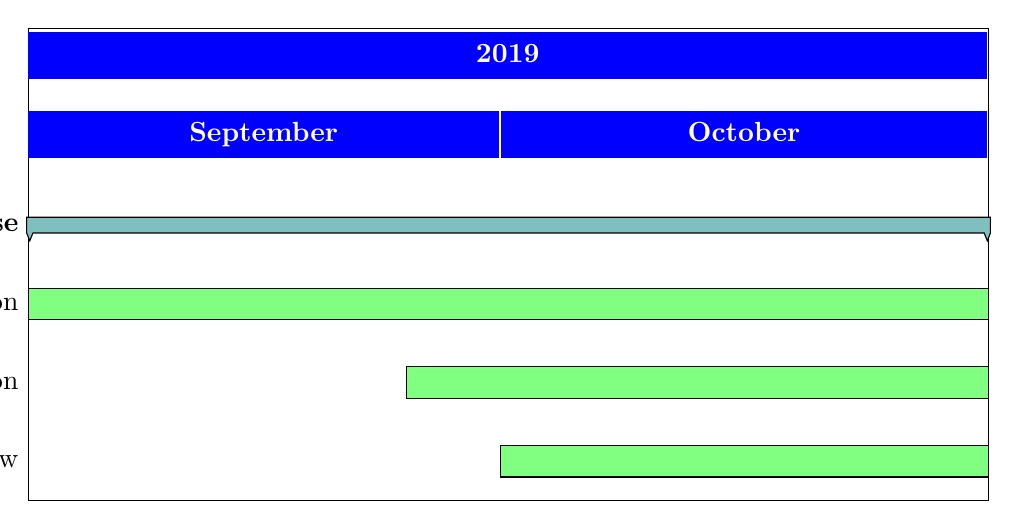
\begin{tikzpicture}
\begin{pgfinterruptboundingbox}
\begin{ganttchart}[Mile/.style={milestone/.append style={fill=red,xscale=5}}, canvas/.append style={alias=frame}, title/.style={fill=blue, draw=none},
		title label font=\color{white}\bfseries,
		time slot format=isodate,
		title right shift=-.1,
		title top shift=.05,
		x unit=2mm
			]{2019-09-01}{2019-10-31}		
     	\gantttitlecalendar{year,month=name} \\
     	
     
       \ganttgroup[group/.append style={draw=black, fill=teal!50}]{Documentation Phase }{2019-09-01}{2019-10-31} \\	
      \ganttbar[bar/.append style={fill=green!50}]{Documenatation}{2019-09-01}{2019-10-31} \\
      \ganttbar[bar/.append style={fill=green!50}]{Presentation}{2019-09-25}{2019-10-31} \\
      \ganttbar[bar/.append style={fill=green!50}]{Review}{2019-10-01}{2019-10-31} 
      
	\end{ganttchart}	
	\end{pgfinterruptboundingbox}
	\useasboundingbox (frame.south west) rectangle (frame.north east);
 \end{tikzpicture} }

\end{figure}

\end{document}